%\documentclass{beamer}
\documentclass[aspectratio=169]{beamer} % took this from the solution
\usetheme{default}
\usecolortheme{crane}
\usepackage{xcolor}


\title{Protocol presentation:\\Tuning strategies for hyperparameters of random forests}
\author{Judith Neve}
\date{
  Department of Methodology and Statistics, UU\\
  Julius Center, UMCU
}

\beamertemplatenavigationsymbolsempty %suppress navigation bar

\begin{document}

%\begin{frame}[plain]
  \titlepage
%\end{frame}
% commenting these out made it start lower on the slide

\begin{frame}{Outline}
    \tableofcontents
\end{frame}

\section{Introduction}

\subsection{What is a random forest?}

\begin{frame}{What is a random forest?}
    \textbf{A single decision tree:}\\
    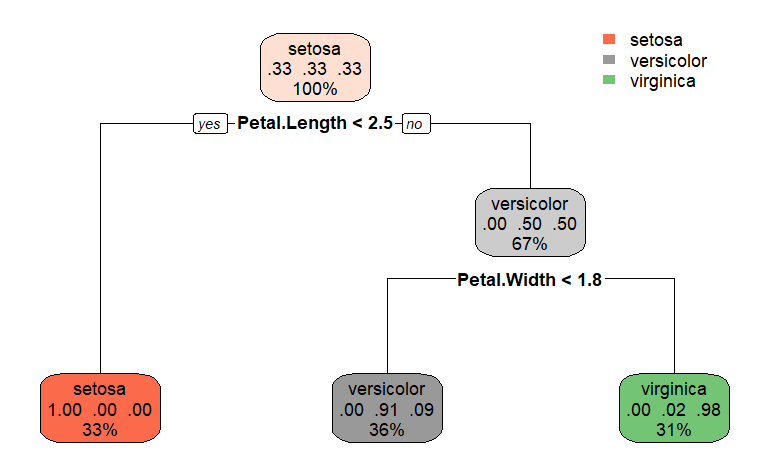
\includegraphics[width = 0.6\textwidth]{Protocol figures/000011.png}
\end{frame}

\begin{frame}{What is a random forest?}
    \textbf{Main idea}: combine many decision trees to classify an observation\\
    \begin{itemize}
        \item For each tree:
        \begin{itemize}
            \item For each split: randomly select $m$ of the candidate predictors
    \end{itemize}
    \item An observation is assigned to a class by majority vote
    \end{itemize}
\end{frame}

\subsection{Hyperparameters}

\begin{frame}{Hyperparameters}
    Lots of settings to choose!\begin{itemize}
        \item Number of trees
        \item Number of candidate predictors
        \item Proportion of the sample used for fitting the tree
        \item Sample with or without replacement
        \item Minimum node size
        \item Split rule
        \item Respect unordered factors
    \end{itemize}
\end{frame}

\subsection{Tuning hyperparameters}

\begin{frame}{Tuning hyperparameters}
    Options:
    \begin{itemize}
        \item Software defaults
        \item Educated guess
        \item Tune them to identify the best ones for the data
    \end{itemize}
\end{frame}

\section{Aims}

\begin{frame}{Aims}
    \begin{enumerate}
        \item Which (combination of) hyperparameters have the most influence on model performance?
        \item Which metric is the most closely related to model performance?
        \item Which hyperparameter search algorithm is the best for model performance and runtime?
    \end{enumerate}
\end{frame}

\section{Data-generating mechanism}

\begin{frame}{Data-generating mechanism: scenarios}
    Varying across the datasets:\begin{itemize}
        \item Number of candidate predictors $p$: 8, 16, 32
        \item Event fraction $EF$: 0.1, 0.3, 0.5
        \item Sample size $n$: 0.5, 1, 2 times the minimum required sample (as defined by Riley, 2020)
    \end{itemize}
    1000 datasets for each scenario $\rightarrow$ 27000 datasets per study\\
    Data simulated under \textbf{logistic regression with strong interactions}
\end{frame}

\begin{frame}{Data-generating mechanism: coefficients}
    For each combination of event fraction $EF$ and number of candidate predictors $p$:\begin{enumerate}
        \item Simulate predictors: 10,000 draws from a $p$-variate normal distribution with mean 0, variance 1, covariance 0.2
        \item Optimise the intercept and slopes to obtain the desired $EF$ and an AUC of 0.7\begin{itemize}
            \item The strength of the effect is the same for all predictors
        \end{itemize}
        \item Using these, optimise $0.25p$ interaction slopes to obtain an AUC of 0.8\begin{itemize}
            \item The strength of the interaction is the same for all interactions
        \end{itemize}
    \end{enumerate}
\end{frame}

\begin{frame}{Data-generating mechanism: data simulation}
    For each scenario:\begin{enumerate}
        \item Simulate predictors: $n$ draws from a $p$-variate normal distribution with mean 0, variance 1, covariance 0.2
        \item Simulate outcomes: $n$ draws from a Bernoulli distribution. The probabilities will be computed using the optimised coefficients and simulated predictors.
    \end{enumerate}
\end{frame}

\section{Estimands}

\begin{frame}{Estimands}
    Model performance:\begin{itemize}
        \item Discrimination (AUC)
        \item Calibration (calibration in the large, calibration slope)
        \item \textbf{For study 3}: runtime
    \end{itemize}
\end{frame}

\section{Methods}

\subsection{Study 1}

\begin{frame}{Methods: Study 1 - hyperparameter combinations}
    Probst et al. (2019): number of candidate predictors and sample fraction have the largest effect on accuracy\\
    \begin{itemize}
        \item All combinations that include these two predictors + no tuning: 33
        \item Fit a random forest tuning each combination on each dataset: 891,000 tuning procedures
    \end{itemize}
    Optimised metric: accuracy\\
    Hyperparameter search algorithm: grid search
\end{frame}

\begin{frame}{Methods: Study 1 - hyperparameter combinations}
    Get a table of the form:\\
    \resizebox{\textwidth}{!}{
    \begin{tabular}{*{8}{|M}|}
         \hline
         \multicolumn{3}{|c|}{Data simulation settings} & Hyperparameters tuned & AUC & Calibration slope & CIL\\
         \hline
         p & Event fraction & Sample size & & & & \\
         \hline
         8 & 0.1 & *0.5 & replace & NA & NA & NA\\
         16 & 0.1 & *0.5 & replace & NA & NA & NA\\
         \hline
         8 & 0.1 & *1 & replace + sample fraction & NA & NA & NA\\
         16 & 0.1 & *1 & replace + sample fraction & NA & NA & NA\\
         \hline
    \end{tabular}}\\
    \begin{enumerate}
        \item Extract top 3 combinations giving the best of each metric
            \item Is there a combination that appears in each metric's top 3? If so, select that combination. If there are multiple, give them each a value (weighted sum of position in top 3 \& performance metric)
    \item If not, take the product of calibration slope (transformed: 1 - absolute deviation from 1) and AUC and select the highest \textbf{such that both metrics are at least as good as the default hyperparameters}
    \end{enumerate}
\end{frame}

\subsection{Study 2}

\begin{frame}{Methods: Study 2 - optimisation metric}
    We tune the hyperparameter combination selected from study 1.\\
    Fit a random forest on each dataset, optimising each of the following candidate metrics:\begin{itemize}
        \item Accuracy [default]
        \item Kappa [as is an option via caret]
        \item Brier score [as is the default in tuneRanger]
        \item AUC [as is an option via tuneRanger]
        \item Logarithmic loss [as is an option via tuneRanger]
    \end{itemize}
    i.e., each dataset is tuned 5 times: 135,000 tuning procedures.\\
    Hyperparameter search algorithm: grid search
\end{frame}

\begin{frame}{Methods: Study 2 - optimisation metric}
    Get a table of the form:\\
    \resizebox{\textwidth}{!}{
    \begin{tabular}{*{8}{|M}|}
         \hline
         \multicolumn{3}{|c|}{Data simulation settings} & Optimisation metric & AUC & Calibration slope & CIL\\
         \hline
         p & Event fraction & Sample size & & & & \\
         \hline
         8 & 0.1 & *0.5 & Accuracy & NA & NA & NA\\
         16 & 0.1 & *0.5 & Accuracy & NA & NA & NA\\
         \hline
         8 & 0.1 & *1 & Kappa & NA & NA & NA\\
         16 & 0.1 & *1 & Kappa & NA & NA & NA\\
         \hline
    \end{tabular}}\\
    \begin{enumerate}
        \item Extract the optimisation metric that leads to the best of each performance metric
        \item Is this consistent? If so, select that combination.
        \item If not, take the product of calibration slope (transformed: 1 - absolute deviation from 1) and AUC and select the highest \textbf{such that both performance metrics are at least as good as that for accuracy}
    \end{enumerate}
\end{frame}

\subsection{Study 3}

\begin{frame}{Methods: Study 3 - hyperparameter search algorithms}
    We tune the hyperparameter combination selected from study 1.\\
    We optimise the metric selected from study 2.
    Fit a random forest on each dataset, using each of the following candidate search algorithms:\begin{itemize}
        \item Model-free search algorithms:\begin{itemize}
            \item Grid search [caret]
            \item Random search [caret]
        \end{itemize}
        \item Bayesian optimisation: SMAC [tuneRanger]
        \item Multifidelity: undefined - have not yet identified an R package
        \item Metaheuristic: genetic algorithm [GA]
    \end{itemize}
    i.e., each dataset is tuned 5 times: 135,000 tuning procedures.
\end{frame}

\begin{frame}{Methods: Study 3 - hyperparameter search algorithms}
    Get a table of the form:\\
    \resizebox{\textwidth}{!}{
    \begin{tabular}{*{9}{|M}|}
         \hline
         \multicolumn{3}{|c|}{Data simulation settings} & Hyperparameter search algorithm & AUC & Calibration slope & CIL & \textbf{Time}\\
         \hline
         p & Event fraction & Sample size & & & & &\\
         \hline
         8 & 0.1 & *0.5 & Grid search & NA & NA & NA & NA\\
         16 & 0.1 & *0.5 & Random search & NA & NA & NA & NA\\
         \hline
         8 & 0.1 & *1 & Grid search & NA & NA & NA & NA\\
         16 & 0.1 & *1 & Random search & NA & NA & NA & NA\\
         \hline
    \end{tabular}}\\
    As of yet unsure how to assess the best one.
\end{frame}

\begin{frame}{Methods: Study 3 - hyperparameter search algorithms}
    Get a figure of the form:
    \centerline{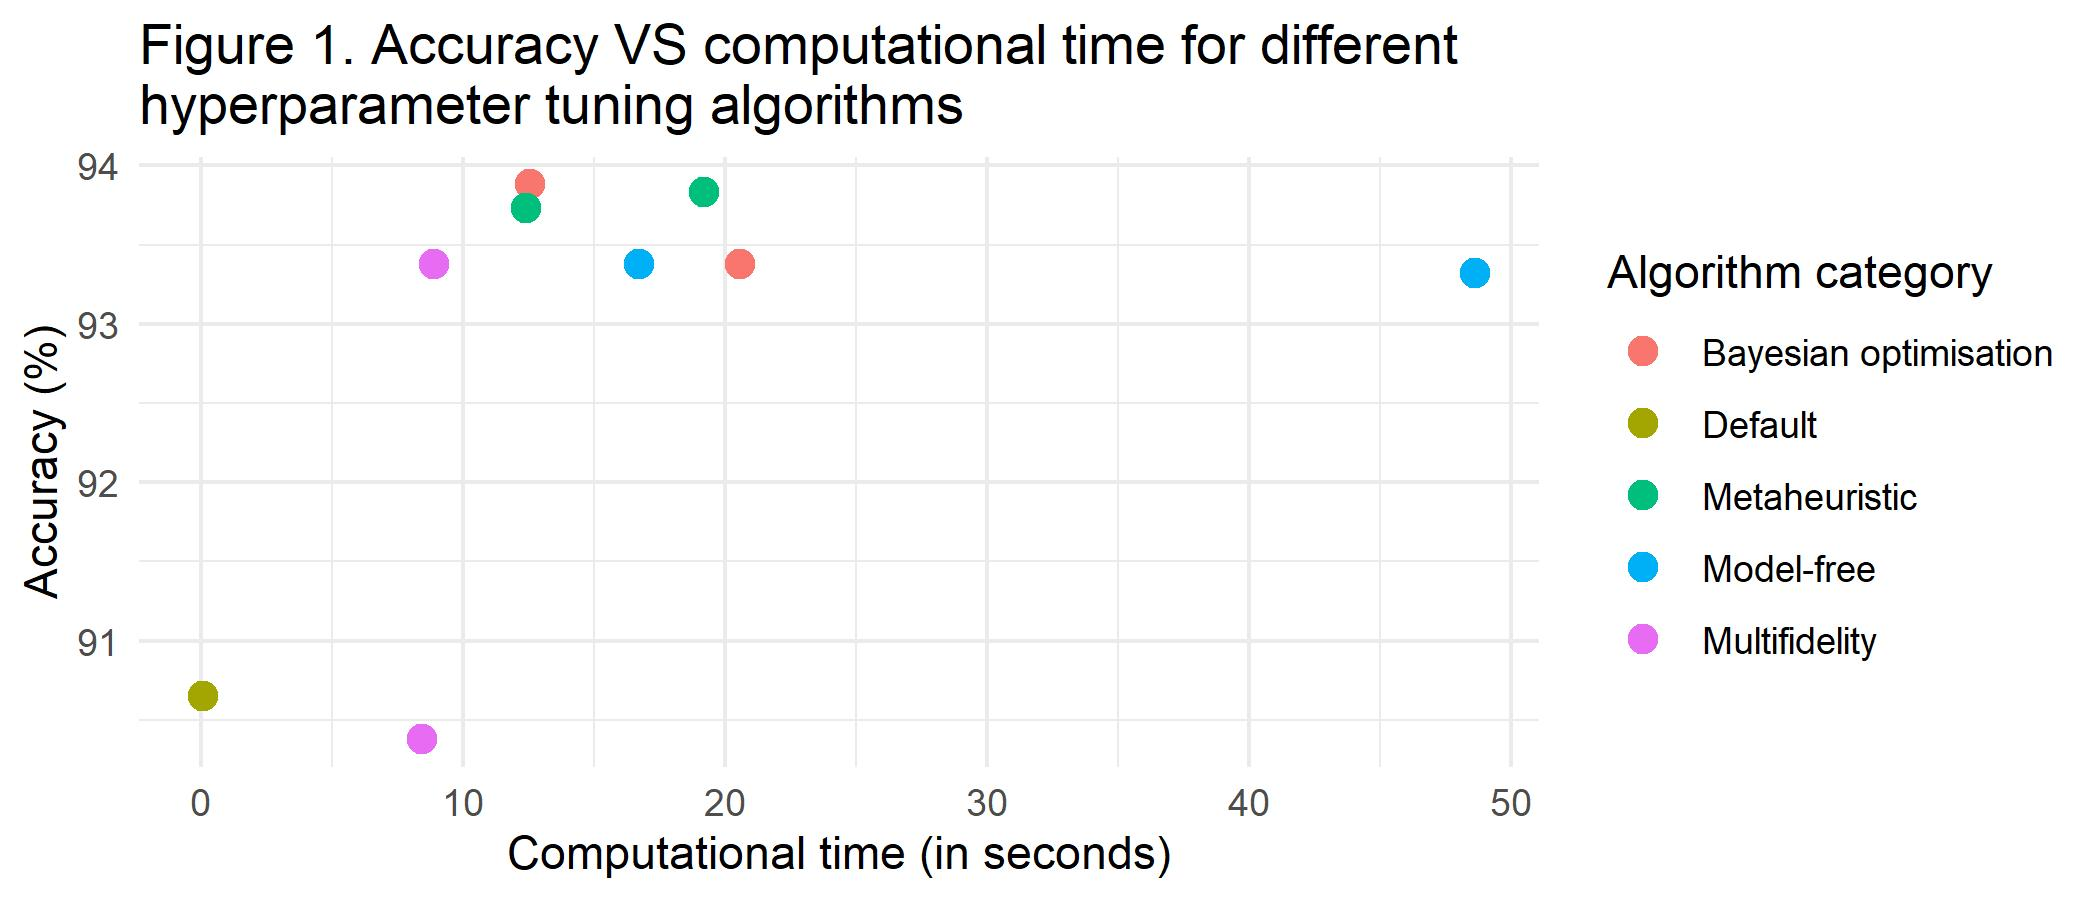
\includegraphics[height = 6cm]{Protocol figures/figure1.jpg}}
\end{frame}

\section{Still to consider}

\begin{frame}{Still to consider}
    \begin{itemize}
        \item Error handling:\begin{itemize}
            \item Degenerate datasets
            \item Non-converging calibration slopes
        \end{itemize}
        \item Study 3:\begin{itemize}
            \item Search algorithms to include
            \item How to draw conclusions
        \end{itemize}
        \item Runtime: pilot studies
    \end{itemize}
\end{frame}

\end{document}